

\subsection{Distros}
\begin{frame}{Distribution?}{Was ist das?}
\begin{columns}
\begin{column}{0.6\textwidth}
Betrieben von: \note{kernel- nicht alleine nutzbar\\}
\begin{itemize}
 \item Community
 \item Firmen
\end{itemize}
Kümmern sich um: \note{passende Softwar zusammenstellen\\} \note{Fehler beheben, Änderungen vorhnehmen (mint, ubuntu, unity)\\}
\begin{itemize}
 \item Pakete
 \item Änderungen/Patches
 \item Hilfe/Support
\end{itemize}
 
 \end{column}
\begin{column}{0.4\textwidth}
 \begin{figure}
 
\includegraphics[height=0.5\textheight]{resources/movers-24402_640.png}
 \end{figure}
\end{column}
\end{columns}
 \end{frame}

\begin{frame}{Distribution}{in:}

 % Michael: Die distros alle wirklich aufzählen?
 \begin{description}
  \item [Pi] Raspian/Kodi/..
  \item [Phone] Android/Sailfish
  \item [Container] Alpine/TinyCore/CoreOS
  \item [Und:] viele embedded Geräte mit speziell angepasstem Linux
 (wie Router, Steuergeräte, Mediengeräte)
 \end{description}

\end{frame}



\begin{frame}{Distribution!}{Zum Beispiel:}
\begin{itemize}%[<+->]
\item Debian
\item Ubuntu
\item Mint
\item Arch
\item openSuse
\item RHEL/Fedora/CentOS 
\item gentoo
\item Puppy/Knoppix 
\item Kali 

\end{itemize}
\end{frame}

\subsection{Oberflächen}
\begin{frame}
\frametitle{Oberflächen}

\note{Gnome3\\}
\begin{figure}
 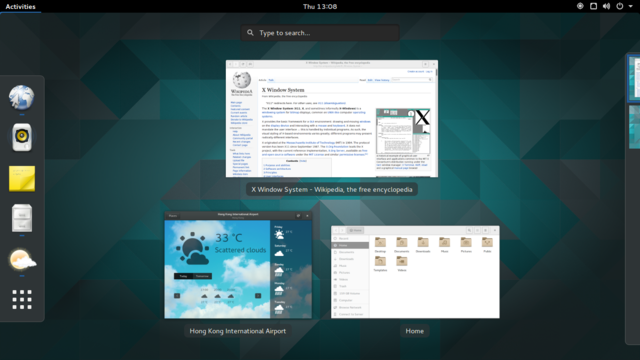
\includegraphics[height=0.7\textheight]{resources/640px-GNOME_Shell.png}
 \end{figure}

\end{frame}
\begin{frame}

\note{unity\\}
\begin{figure}
 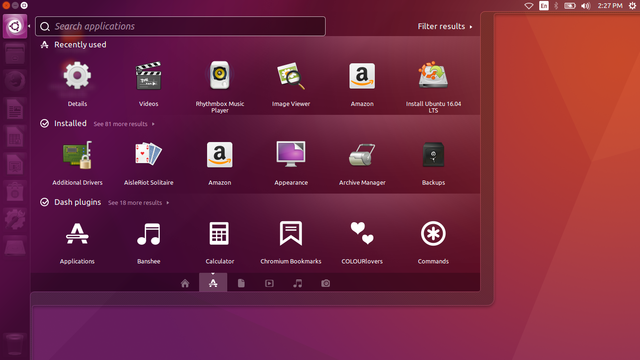
\includegraphics[height=0.7\textheight]{resources/640px-App_Lens_on_Ubuntu.png}
 \end{figure}
\end{frame}

\begin{frame}

\note{KDE/Plasma\\}
\begin{figure}
 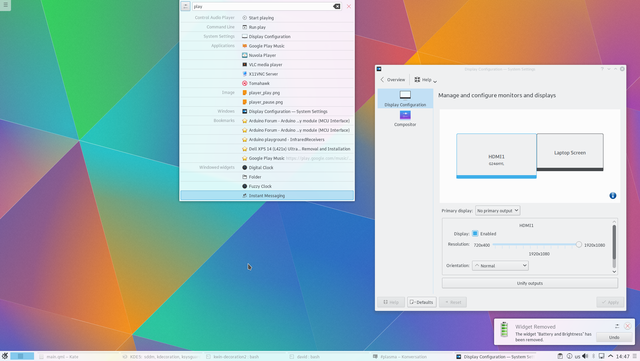
\includegraphics[height=0.7\textheight]{resources/640px-Kscreen-krunner.png}
 \end{figure}


\end{frame}


%\subsection{Programme}
\begin{frame}[allowframebreaks]{Programme}{Für Desktop}
 
 %\begin{tabular}{lp{5cm}}
 %Kategorie& Software \\ \hline
 
\hspace{1cm}

\begin{description}[style=nextline]

 \item [Browser] {\bf Firefox}, Chromium, Vivaldi, Opera, Tor

 \item [Office] {\bf LibreOffice}, Kile (\LaTeX), \TeX maker

 \item [Email Clients] {\bf Thunderbird}, Icedove, Evolution 

 \item [Messenger] Pidgin, Empathy, HexChat, Telegram

 \item [VoIP] Mumble, Ring, Tox

 \item [Synchronisation] {\bf Nextcloud}, Owncloud, Seafile
\pagebreak 
 \item [IDEs] {\bf Eclipse}, IntelliJ, NetBeans, Atom, VI(M)

 \item [Medien]{\bf VLC}, Audacity, Rythmbox, Totem

 \item [Grafik] {\bf GIMP}, Blender,  Inkscape

 \item [System] {\bf Wireshark}, GParted, Boabab, Filezilla

 \item [Torrents] Transmission 

 \item [alles] DAS TERMINAL 

\end{description}
 \end{frame}




